\resizebox{0.5\textwidth}{!}{\begin{tikzpicture} [myv/.style={circle, draw, inner sep=8pt,line width=0.8mm},myv1/.style={circle, draw, inner sep=0pt,color=white},myv2/.style={rectangle, draw, dotted,  inner sep=2pt,line width = 0.8mm}]
 % \node [label=above: $\Large{r}$](z)  at (0,4) {};

  \node[myv] (a) at (-4,1) {};
  \node[myv] (b) at (-4,3) {};
  \node[myv] (c) at (2,1) {};
  \node[myv] (d) at (2,3) {};
 % \node[circle, draw, inner sep=5pt] (d) at (4,2) {};
  \node[myv] (e) at (8,1) {};
  \node[myv] (f) at (8,3) {};
  
    \draw[line width=0.8mm]  (a) -- (b);
    \draw[line width=0.8mm] (b) -- (c);
    \draw[line width=0.8mm] (c) -- (d);
    \draw[line width=0.8mm] (d) -- (e);
    \draw[line width=0.8mm] (e) -- (f);
    \draw[line width=0.8mm] (e) -- (b);
    
    
    \node (g) at (-4,-4) { {\resizebox{0.25\textwidth}{!}{\begin{tikzpicture}[myv/.style={circle, draw, inner sep=8pt},myv1/.style={circle, draw, inner sep=0pt,color=white},myv2/.style={rectangle, draw,dotted,inner sep=0pt,line width = 0.5mm}]
 % \node [label=above: $\Large{r}$](z)  at (0,4) {};

  \node[myv] (a) at (0,4) {};
  \node[myv] (b) at (-2,2) {};
  \node[myv] (c) at (2,2) {};

  \node[myv] (d) at (-3,0) {};
  \node[myv] (e) at (-1,0) {};
  \node[myv] (f) at (1,0) {};
  \node[myv] (g) at (3,0) {};

  \node[myv] (h) at (-3,-2) {};
  \node[myv] (i) at (-1,-2) {};
  \node[myv] (j) at (1,-2) {};
  \node[myv] (k) at (3,-2) {};
   \node[myv1] (l)  at (3,-2.5) {};
   \node[myv1] (m)  at (3,-3) {};
  
    \draw (a) -- (b);
    \draw (a) -- (c);
    \draw (b) -- (d);
    \draw (b) -- (e);
    \draw (c) -- (f);
    \draw (c) -- (g);
    \draw (d) -- (h);
    \draw (d) -- (i);
    \draw (e) -- (h);
    \draw (e) -- (i);
    \draw (f) -- (j);
    \draw (f) -- (k);
    \draw (g) -- (j);
    \draw (g) -- (k);
    \draw (i) to [bend right=20] (j);
    \draw (h) to [bend right=20] (k);

   

\end{tikzpicture}}
}};
    \node[myv2] [fit=  (g), inner xsep=0.5ex, inner ysep=0.5ex] {};
    \node  (h) at (2,-4) {\resizebox{0.25\textwidth}{!}{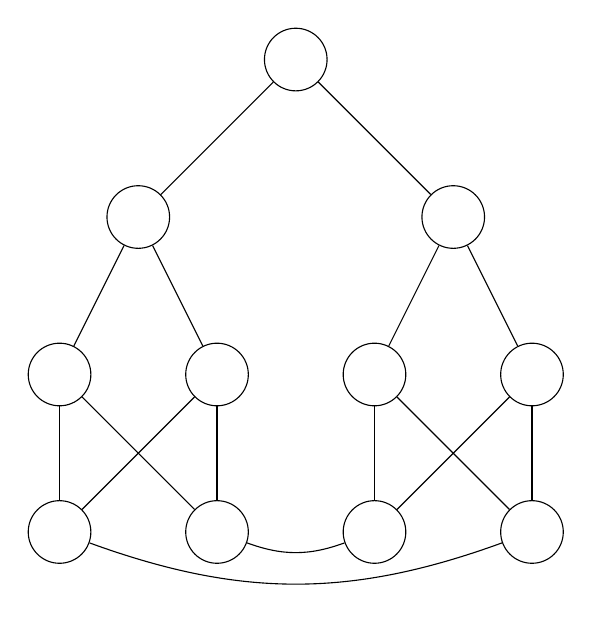
\begin{tikzpicture}[myv/.style={circle, draw, inner sep=8pt},myv1/.style={circle, draw, inner sep=0pt,color=white},myv2/.style={rectangle, draw,dotted,inner sep=0pt,line width = 0.5mm}]
 % \node [label=above: $\Large{r}$](z)  at (0,4) {};

  \node[myv] (a) at (0,4) {};
  \node[myv] (b) at (-2,2) {};
  \node[myv] (c) at (2,2) {};

  \node[myv] (d) at (-3,0) {};
  \node[myv] (e) at (-1,0) {};
  \node[myv] (f) at (1,0) {};
  \node[myv] (g) at (3,0) {};

  \node[myv] (h) at (-3,-2) {};
  \node[myv] (i) at (-1,-2) {};
  \node[myv] (j) at (1,-2) {};
  \node[myv] (k) at (3,-2) {};
   \node[myv1] (l)  at (3,-2.5) {};
   \node[myv1] (m)  at (3,-3) {};
  
    \draw (a) -- (b);
    \draw (a) -- (c);
    \draw (b) -- (d);
    \draw (b) -- (e);
    \draw (c) -- (f);
    \draw (c) -- (g);
    \draw (d) -- (h);
    \draw (d) -- (i);
    \draw (e) -- (h);
    \draw (e) -- (i);
    \draw (f) -- (j);
    \draw (f) -- (k);
    \draw (g) -- (j);
    \draw (g) -- (k);
    \draw (i) to [bend right=20] (j);
    \draw (h) to [bend right=20] (k);

   

\end{tikzpicture}}
};
    \node[myv2]   [fit=  (h), inner xsep=0.5ex, inner ysep=0.5ex] {};
    \node  (i) at (8,-4) {\resizebox{0.25\textwidth}{!}{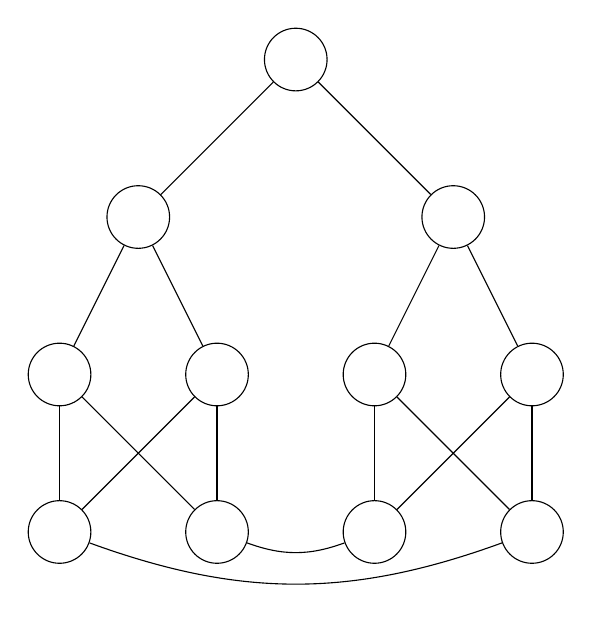
\begin{tikzpicture}[myv/.style={circle, draw, inner sep=8pt},myv1/.style={circle, draw, inner sep=0pt,color=white},myv2/.style={rectangle, draw,dotted,inner sep=0pt,line width = 0.5mm}]
 % \node [label=above: $\Large{r}$](z)  at (0,4) {};

  \node[myv] (a) at (0,4) {};
  \node[myv] (b) at (-2,2) {};
  \node[myv] (c) at (2,2) {};

  \node[myv] (d) at (-3,0) {};
  \node[myv] (e) at (-1,0) {};
  \node[myv] (f) at (1,0) {};
  \node[myv] (g) at (3,0) {};

  \node[myv] (h) at (-3,-2) {};
  \node[myv] (i) at (-1,-2) {};
  \node[myv] (j) at (1,-2) {};
  \node[myv] (k) at (3,-2) {};
   \node[myv1] (l)  at (3,-2.5) {};
   \node[myv1] (m)  at (3,-3) {};
  
    \draw (a) -- (b);
    \draw (a) -- (c);
    \draw (b) -- (d);
    \draw (b) -- (e);
    \draw (c) -- (f);
    \draw (c) -- (g);
    \draw (d) -- (h);
    \draw (d) -- (i);
    \draw (e) -- (h);
    \draw (e) -- (i);
    \draw (f) -- (j);
    \draw (f) -- (k);
    \draw (g) -- (j);
    \draw (g) -- (k);
    \draw (i) to [bend right=20] (j);
    \draw (h) to [bend right=20] (k);

   

\end{tikzpicture}}
};
    \node[myv2]   [fit=  (i), inner xsep=0.5ex, inner ysep=0.5ex] {};
    \node  (j) at (-4,8) {\resizebox{0.35\textwidth}{!}{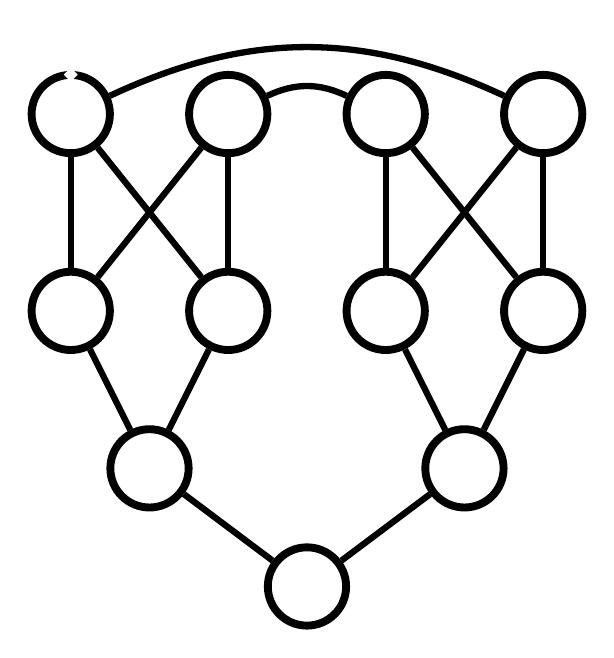
\begin{tikzpicture}[rotate=180,myv/.style={circle, draw, inner sep=10pt,line width=1mm},myv1/.style={circle, draw, inner sep=0pt,color=white,line width=1mm},myv2/.style={rectangle, draw,dotted,inner sep=0pt,line width = 0.5mm}]
 % \node [label=above: $\Large{r}$](z)  at (0,4) {};

  \node[myv] (a) at (0,4) {};
  \node[myv] (b) at (-2,2.5) {};
  \node[myv] (c) at (2,2.5) {};

  \node[myv] (d) at (-3,0.5) {};
  \node[myv] (e) at (-1,0.5) {};
  \node[myv] (f) at (1,0.5) {};
  \node[myv] (g) at (3,0.5) {};

  \node[myv] (h) at (-3,-2) {};
  \node[myv] (i) at (-1,-2) {};
  \node[myv] (j) at (1,-2) {};
  \node[myv] (k) at (3,-2) {};
   \node[myv1] (l)  at (3,-2.5) {};
   \node[myv1] (m)  at (3,-3) {};

    \draw[line width=0.8mm] (a) -- (b);
    \draw[line width=0.8mm] (a) -- (c);
    \draw[line width=0.8mm] (b) -- (d);
    \draw[line width=0.8mm] (b) -- (e);
    \draw[line width=0.8mm] (c) -- (f);
    \draw[line width=0.8mm] (c) -- (g);
    \draw[line width=0.8mm] (d) -- (h);
    \draw[line width=0.8mm] (d) -- (i);
    \draw[line width=0.8mm] (e) -- (h);
    \draw[line width=0.8mm] (e) -- (i);
    \draw[line width=0.8mm] (f) -- (j);
    \draw[line width=0.8mm] (f) -- (k);
    \draw[line width=0.8mm] (g) -- (j);
    \draw[line width=0.8mm] (g) -- (k);
    \draw[line width=0.8mm] (i) to [bend right=25] (j);
    \draw[line width=0.8mm] (h) to [bend right=25] (k);

\end{tikzpicture}}};
    \node[myv2]   [fit=  (j), inner xsep=0.5ex, inner ysep=0.5ex] {};
    \node   (k) at (2,8) {\resizebox{0.35\textwidth}{!}{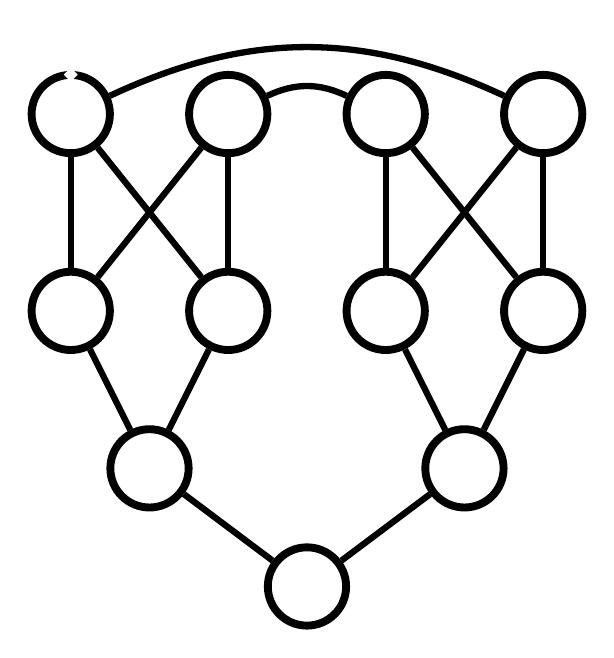
\begin{tikzpicture}[rotate=180,myv/.style={circle, draw, inner sep=10pt,line width=1mm},myv1/.style={circle, draw, inner sep=0pt,color=white,line width=1mm},myv2/.style={rectangle, draw,dotted,inner sep=0pt,line width = 0.5mm}]
 % \node [label=above: $\Large{r}$](z)  at (0,4) {};

  \node[myv] (a) at (0,4) {};
  \node[myv] (b) at (-2,2.5) {};
  \node[myv] (c) at (2,2.5) {};

  \node[myv] (d) at (-3,0.5) {};
  \node[myv] (e) at (-1,0.5) {};
  \node[myv] (f) at (1,0.5) {};
  \node[myv] (g) at (3,0.5) {};

  \node[myv] (h) at (-3,-2) {};
  \node[myv] (i) at (-1,-2) {};
  \node[myv] (j) at (1,-2) {};
  \node[myv] (k) at (3,-2) {};
   \node[myv1] (l)  at (3,-2.5) {};
   \node[myv1] (m)  at (3,-3) {};

    \draw[line width=0.8mm] (a) -- (b);
    \draw[line width=0.8mm] (a) -- (c);
    \draw[line width=0.8mm] (b) -- (d);
    \draw[line width=0.8mm] (b) -- (e);
    \draw[line width=0.8mm] (c) -- (f);
    \draw[line width=0.8mm] (c) -- (g);
    \draw[line width=0.8mm] (d) -- (h);
    \draw[line width=0.8mm] (d) -- (i);
    \draw[line width=0.8mm] (e) -- (h);
    \draw[line width=0.8mm] (e) -- (i);
    \draw[line width=0.8mm] (f) -- (j);
    \draw[line width=0.8mm] (f) -- (k);
    \draw[line width=0.8mm] (g) -- (j);
    \draw[line width=0.8mm] (g) -- (k);
    \draw[line width=0.8mm] (i) to [bend right=25] (j);
    \draw[line width=0.8mm] (h) to [bend right=25] (k);

\end{tikzpicture}}};
    \node[myv2]   [fit=  (k), inner xsep=0.5ex, inner ysep=0.5ex] {};
    \node   (l) at (8,8) {\resizebox{0.35\textwidth}{!}{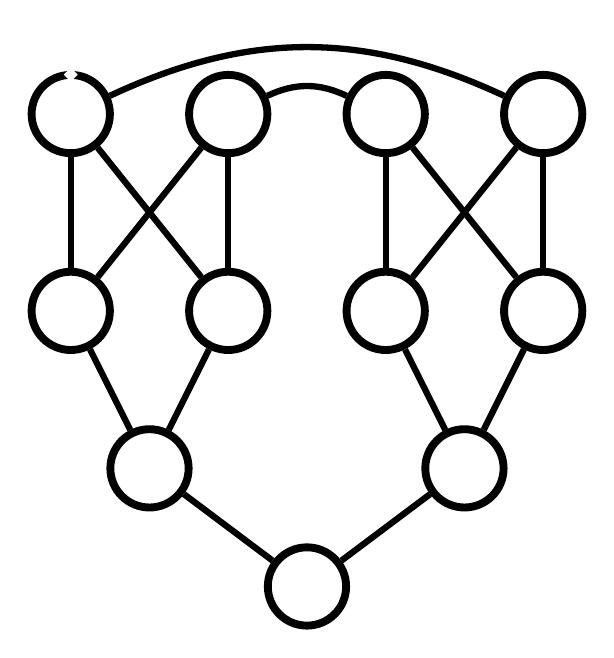
\begin{tikzpicture}[rotate=180,myv/.style={circle, draw, inner sep=10pt,line width=1mm},myv1/.style={circle, draw, inner sep=0pt,color=white,line width=1mm},myv2/.style={rectangle, draw,dotted,inner sep=0pt,line width = 0.5mm}]
 % \node [label=above: $\Large{r}$](z)  at (0,4) {};

  \node[myv] (a) at (0,4) {};
  \node[myv] (b) at (-2,2.5) {};
  \node[myv] (c) at (2,2.5) {};

  \node[myv] (d) at (-3,0.5) {};
  \node[myv] (e) at (-1,0.5) {};
  \node[myv] (f) at (1,0.5) {};
  \node[myv] (g) at (3,0.5) {};

  \node[myv] (h) at (-3,-2) {};
  \node[myv] (i) at (-1,-2) {};
  \node[myv] (j) at (1,-2) {};
  \node[myv] (k) at (3,-2) {};
   \node[myv1] (l)  at (3,-2.5) {};
   \node[myv1] (m)  at (3,-3) {};

    \draw[line width=0.8mm] (a) -- (b);
    \draw[line width=0.8mm] (a) -- (c);
    \draw[line width=0.8mm] (b) -- (d);
    \draw[line width=0.8mm] (b) -- (e);
    \draw[line width=0.8mm] (c) -- (f);
    \draw[line width=0.8mm] (c) -- (g);
    \draw[line width=0.8mm] (d) -- (h);
    \draw[line width=0.8mm] (d) -- (i);
    \draw[line width=0.8mm] (e) -- (h);
    \draw[line width=0.8mm] (e) -- (i);
    \draw[line width=0.8mm] (f) -- (j);
    \draw[line width=0.8mm] (f) -- (k);
    \draw[line width=0.8mm] (g) -- (j);
    \draw[line width=0.8mm] (g) -- (k);
    \draw[line width=0.8mm] (i) to [bend right=25] (j);
    \draw[line width=0.8mm] (h) to [bend right=25] (k);

\end{tikzpicture}}};
    \node[myv2]   [fit=  (l), inner xsep=0.5ex, inner ysep=0.5ex] {};

   \draw[line width=0.8mm] (-4, -1.25) -- (-4,0.7);
   \draw[line width=0.8mm] (2,-1.15) -- (-3.65,1.0);
   \draw[line width=0.8mm] (2.25,0.75) -- (8, -1.15);
   \draw[line width=0.8mm] (-4,5.15) -- (2,3.35);
   \draw[line width=0.8mm] (2, 5.15) -- (8,3.35);
   \draw[line width=0.8mm] (8,3.35) -- (8,5.2);

\end{tikzpicture}}